For a given sequence as a learning process, the \textit{tournois} are indexed for each \textit{colonne} at the level of the class MLT, whose order will be defined by the slot \texttt{cover-value}. The \textit{tournois} (with \texttt{remanence}\footnote{The remanence means if we consider the \textit{tournois} with the cover-value as they are recorded (i.e. the order of the \textit{tournois}) or if we only consider the arcs.} \textit{true}) and the arcs constituting the \textit{tournois} (with \texttt{remanence} \textit{nil}) will be retained in a separate hash table associated with each SOM.

Note that \texttt{cover-value} must imperatively be an integer and greater than or equal to 3 (since a \textit{tournoi} is defined only from 3 nodes).

\bigskip

The \textit{microcolonnes} of each SOM are listed and indexed according to their symbolic representation -- i.e. the type of information conveyed, triggered by \textit{stimuli} -- in the slot \texttt{fanaux-list} as a list of neurons. In other words, the 
\textit{microcolonnes} is the SOM reduced to the fanaux-list.
\bigskip

\begin{lstlisting}[language=N3]
(update-fanaux SOMNAME <int>) ; if needed
(dolist (k SEQUENCCE)
  (setf (input SOMNAME) k)
  (learn SOMNAME :seq t))
\end{lstlisting}

\bigskip

N3 allows if needed to update by surjection\footnote{The surjection algorithm consists to explore the distance matrix of the `new-fanaux-list' from `the old-fanaux-list' in order to retain only the neurons with the smallest distance per row and by column. The conjunction of the last two is listed according to the index of the `old-fanaux-list', adding if necessary the intermediate distances.\label{surj}} the fanaux-list with the method \glspl{update-fanaux} according to the `old-fanaux-list' -- if this latest is not nil. This means the modification of the arcs (at the SOM level) and of the involved edges (at the AREA level) if applicable. Mind that this will inevitably lead to an alteration -- more or less significant depending on the degree of change -- of what has been learned so far.

\bigskip
There are two ways to read the acquis of the MLT. The first one consists to retrace one (or more) \textit{tournoi(s)} from a partial sequence temporally ordered according to the remanence or not. The method \glspl{locate-tournoi} allows to do that and gives as result a list of potential \textit{tournoi(s)} sorted according to their weight. 

\bigskip
\begin{lstlisting}[language=N3]
(locate-tournoi SOMNAME '(3 ? 0) :remanence nil)
; ((0.28400004 (3 2 0)) (0.22000018 (3 3 0)) (0.2 (3 0 0)) (0.15999967 (3 1 0)) (0.13600005 (3 4 0)))
(locate-tournoi SOMNAME '(3 ? 0) :remanence t)
; ((0.5 (3 2 0)) (0.5 (3 3 0)))
\end{lstlisting}
\bigskip

Note that with the remanence case, the given \textit{tournoi} is compared with the learned \textit{tournois} of MLT, and each match is retained with its weight, then the sum of all these weights is normalised. In the case of the length of the given \textit{tournoi} is superior to the \texttt{cover-value}, this one is decomposed as follow: for instance consider the tournoi \texttt{(a b c d e)} and the \texttt{cover-value} equal to 3, then the computation is done on \texttt{(a b c) (b c d)} and  \texttt{(c d e)}.

\smallskip

Also, to limit the search space -- which increases exponentially -- each \textit{tournoi} composed with only wild cards is avoided. In that case, there are two undocumented functions to do the job as \texttt{all-tournoi} -- which lists all the possible \textit{tournois} according to a given order and the remanence as keys -- and \texttt{rnd-tournoi} -- which chooses randomly but weighted from the previous result.

\bigskip

The second one expresses the previous result in terms of probability by `postpended' a wild card. 
Thus, the method \glspl{next-event-probability} allows to compute the probability of occurrences for a \textit{fanal} to occur after a given subsequence of \textit{fanaux} -- as a list of indexed \textit{fanaux} temporally ordered (with the possibility to add `?' as a wild card).

\smallskip

Then, the purpose of this function allows to estimate an occurrence -- with the key \texttt{:result :eval} (set by default) -- through the key function \texttt{:compute} (set with the function \texttt{rnd-weight} by default). 

The function \texttt{rnd-weight} allows to choose a number at random between $0$ and $1$ such as this interval is conformed to the ordered repartition of probabilities (see the coloured stripes under the next code snippets).

\bigskip

\begin{lstlisting}[language=N3]
(next-event-probability '(3 ? 0) SOMNAME :remanence nil     :result :verbose) 
; 2 => 30.749 %
; 3 => 22.460 %
; 0 => 16.756 %
; 1 => 16.043 %
; 4 => 13.993 %
\end{lstlisting}

\bigskip

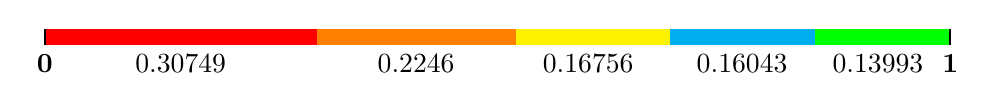
\begin{tikzpicture}[xscale=11.5]
\draw[-][draw=red, line width=2mm] (0,0) -- (.3,0);
\draw[-][draw=orange, line width=2mm]  (.3,0) -- (.52,0);
\draw[-][draw=yellow, line width=2mm] (.52,0) -- (.69,0);
\draw[-][draw=cyan, line width=2mm] (.69,0) -- (.85,0);
\draw[-][draw=green, line width=2mm] (.85,0) -- (1,0);
\draw [thick] (0,-.1) node[below]{\textbf{0}} -- (0,0.1);
\draw [thick] (0.15,-.1) node[below]{$0.30749$} ;
\draw [thick] (0.41,-.1) node[below]{$0.2246$} ;
\draw [thick] (0.6,-.1) node[below]{$0.16756$} ;
\draw [thick] (0.77,-.1) node[below]{$0.16043$} ;
\draw [thick] (0.92,-.1) node[below]{$0.13993$} ;
\draw [thick] (1,-.1) node[below]{\textbf{1}} -- (1,0.1);
\end{tikzpicture}

\bigskip

\begin{lstlisting}[language=N3]
(next-event-probability '(3 ? 0) SOMNAME :remanence t       :result :verbose) 
; 0 => 28.571 %
; 2 => 23.810 %
; 1 => 19.048 %
; 3 => 19.048 %
; 4 =>  9.524 %
\end{lstlisting}

\bigskip

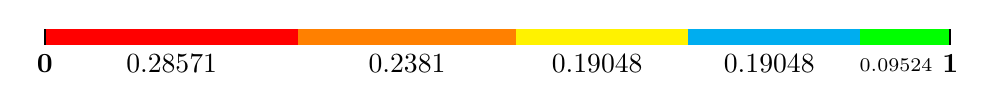
\begin{tikzpicture}[xscale=11.5]
\draw[-][draw=red, line width=2mm] (0,0) -- (.28,0);
\draw[-][draw=orange, line width=2mm]  (.28,0) -- (.52,0);
\draw[-][draw=yellow, line width=2mm] (.52,0) -- (.71,0);
\draw[-][draw=cyan, line width=2mm] (.71,0) -- (.9,0);
\draw[-][draw=green, line width=2mm] (.9,0) -- (1,0);
\draw [thick] (0,-.1) node[below]{\textbf{0}} -- (0,0.1);
\draw [thick] (0.14,-.1) node[below]{$0.28571$} ;
\draw [thick] (0.4,-.1) node[below]{$0.2381$} ;
\draw [thick] (0.61,-.1) node[below]{$0.19048$} ;
\draw [thick] (0.8,-.1) node[below]{$0.19048$} ;
\draw [thick] (0.94,-.15) node[below]{{\scriptsize $0.09524$}} ;
\draw [thick] (1,-.1) node[below]{\textbf{1}} -- (1,0.1);
\end{tikzpicture}




